\chapter{Modelle}
\section{Szenarios}
\subsection{Überwachung und Messung an einem Versuchsaufbau}
Angenommen jemand hat einen Versuchsaufbau mit mehreren Temperatursensoren gleichen Types aufgebaut und will damit seine Wohnung, über die Dauer einer Woche, überwachen. Der Aufbau ist relativ schnell bewältigt und das größte Problem ist die Flut an Daten die bewältigt werden muss, wenn jede Minute ein Wert pro Sensor gespeichert werden soll. Darüber hinaus sollen die Daten so hinterlegt werden, dass eine spätere Auswertung, evtl. auch durch Dritte, nach gängigen Normen vorgenommen werden kann. Der Nutzer hat in seinem beruflichen Umfeld bereits Erfahrungen mit Elektrotechnik gesammelt und ist geübt im Umgang mit Computern und der Bedienung von Anwendungen.

Der Aufbau ist abgeschlossen und er sucht nur noch nach einer Software die seinen Bedürfnissen entspricht. Hier kommt die zu entwickelnde Software ins Spiel. Er startet die Software und konfiguriert  seine Messung mit Hilfe des \glslink{Wizard}{Wizards} nach seinen Vorstellungen. Er will das die Werte nicht nur generisch "A1", "`A2"' und so weiter heißen, sondern entsprechender des Raumes in dem sich der Sensor befindet beschriftet werden. Sofort sieht er in dem Wizard diese Option und trägt die Beschriftung der Pins in die vorgesehenen Textboxen ein. Da die Sensoren nur ein analoges Signal im Rahmen von 0 bis 5 Volt ausgeben und dieses Signal noch in Grad Celsius umgewandelt werden muss trägt er zu jedem Pin noch die entsprechende Übertragungsfunktion ein. Nachdem dies geschehen ist, geht er in dem Wizard eine Schritt weiter und bekommt die Möglichkeit die digitalen Pins des Arduinos zu Steuern. Er entscheidet sich gegen die Nutzung. Es sollen lediglich Daten gemessen und geloggt werden. Auf der letzten Seite des Wizards bekommt er die Optionen zu Einrichtung des \acrshort{CSV}-Loggers. Da er die Software auf einer deutschsprachigen Maschine betreibt und die anschließende Auswertung auch in einer deutschsprachigen Tabellenbearbeitungssoftware geschehen wird gibt er an welche Tausendertrenner und ähnliches verwendet werden sollen. Der Wizard hat ihm allerdings auf Grund der verwendeten System-Einstellungen diesen Vorschlag bereits unterbreitet. Der Nutzer gibt nur noch an das er sowohl die umgerechneten Temperaturen und die Spannungswerte in dem Log hinterlegt haben möchte. 

Nach dem die Konfiguration abgeschlossen ist, muss noch der Arduino-Sketch mittels der Arduino eigenen \acrshort{IDE} installiert werden. Ist dies erfolgt kann die Messung beginnen. Der Nutzer bekommt nun in Echtzeit die gemessenen Werte angezeigt. Er kann selektiv nur einen oder mehrere Werte anzeigen lassen und zwischen den Spannungswerten und den umgerechneten Werten auswählen. Zusätzlich kann er sich noch eine Tendenz einblenden lassen, um etwa zu sehen wann und wo er vergessen hat ein Fenster zu schließen und somit der Raum auskühlt. 

Nun da die Messung läuft kann er sich anderen Dingen zuwenden und ggf. ab und zu nachschauen ob es interessante Veränderungen in den gemessen Werten gibt.
Nach Ablauf der einen Woche beendet er die Messung und kann nun die Werte mit Hilfe einer anderen Software genauer überprüfen.
\subsection{Steuerung und Messung an einem Versuchsaufbau}
Angenommen ein Nutzer verfügt über einen Versuchsaufbau um einen Luftentfeuchter zu betreiben. Dieser Aufbau benötigt die Option den Entfeuchtungsprozess ein und auszuschalten je nach Feuchtigkeit der ihn umgebenden Luft. Er hat eine genaue Vorstellung der Grenzwerte zum ein und ausschalten des Entfeuchters und beginnt folglich mit der Konfiguration einer entsprechenden Messung in der Software. Den benötigten Arduino hat er bereits an den Entfeutcher angeschlossen und alle notwendigen Pins mit ihren Konterparts verbunden. Die Software des Arduinos hat er mit Hilfe der \acrshort{IDE} installiert. Geleitet wurde er dabei von einer, der Software beiliegenden, Anleitung. Nun kann er die Software starten und mit der Konfiguration beginnen.
Mit Hilfe des Wizards benennt er die Signale die über die analogen Schnittstellen seines Arduinos gemessen werden und versieht sie zu gleich mit der von Sensorhersteller angegebenen Übertragungsfunktion. Hat er diesen Schritt beendet, kann er auf der nächsten Seite des Wizards Bedingungen definieren um die Pumpe des Entfeuchters ein bzw. auszuschalten. Er verknüpft dafür die entsprechenden analogen Signale, wahlweise die Spannungswerte oder die übersetzten Werte mit einem entsprechenden digitalen Pin und bestimmt das Verhalten bei bestimmten Werten. Der Nutzer entscheidet sich den Entfeuchter abzuschalten wenn der relative Feutchtigkeitswert unter 50\% fällt. Diesen Wert hat er aus einem Wohnmagazin entnommen, mit dem Versprechend, dass diese Feuchtigkeit bei Wohn und Arbeitsräumen als angenehm empfunden wird bei einer Raumtemperatur von etwa 20 Grad Celsius. 

Nachdem die Bedingungen definieren sind, sieht der Nutzer die letzte Seite des Wizards und kann dort den Logger einstellen, da er eine gewissen Neugierde über den Feutigkeitsverlauf in dem Raum empfindet entscheidet er sich die Werte auch gleich mit zu loggen, in einem Rhythmus von 10 Minuten. 

Sobald diese letzte Option bearbeitet wurde startet der Nutzer die Messung. Nach einiger Zeit, etwa 3 Tagen, kommt er zurück und schaut sich die bis dahin gemessenen Werte an. Eine Auswertung kann er nun mit einem anderen Programm vollziehen und ggf. Konsequenzen in seinem Lüftungsverhalten o.ä. vornehmen.
\section{Use case model}
Dieses Use case Diagramm zeigt die dem Nutzer zu Verfügung stehen Optionen.
\begin{figure}[H]
 \centering
 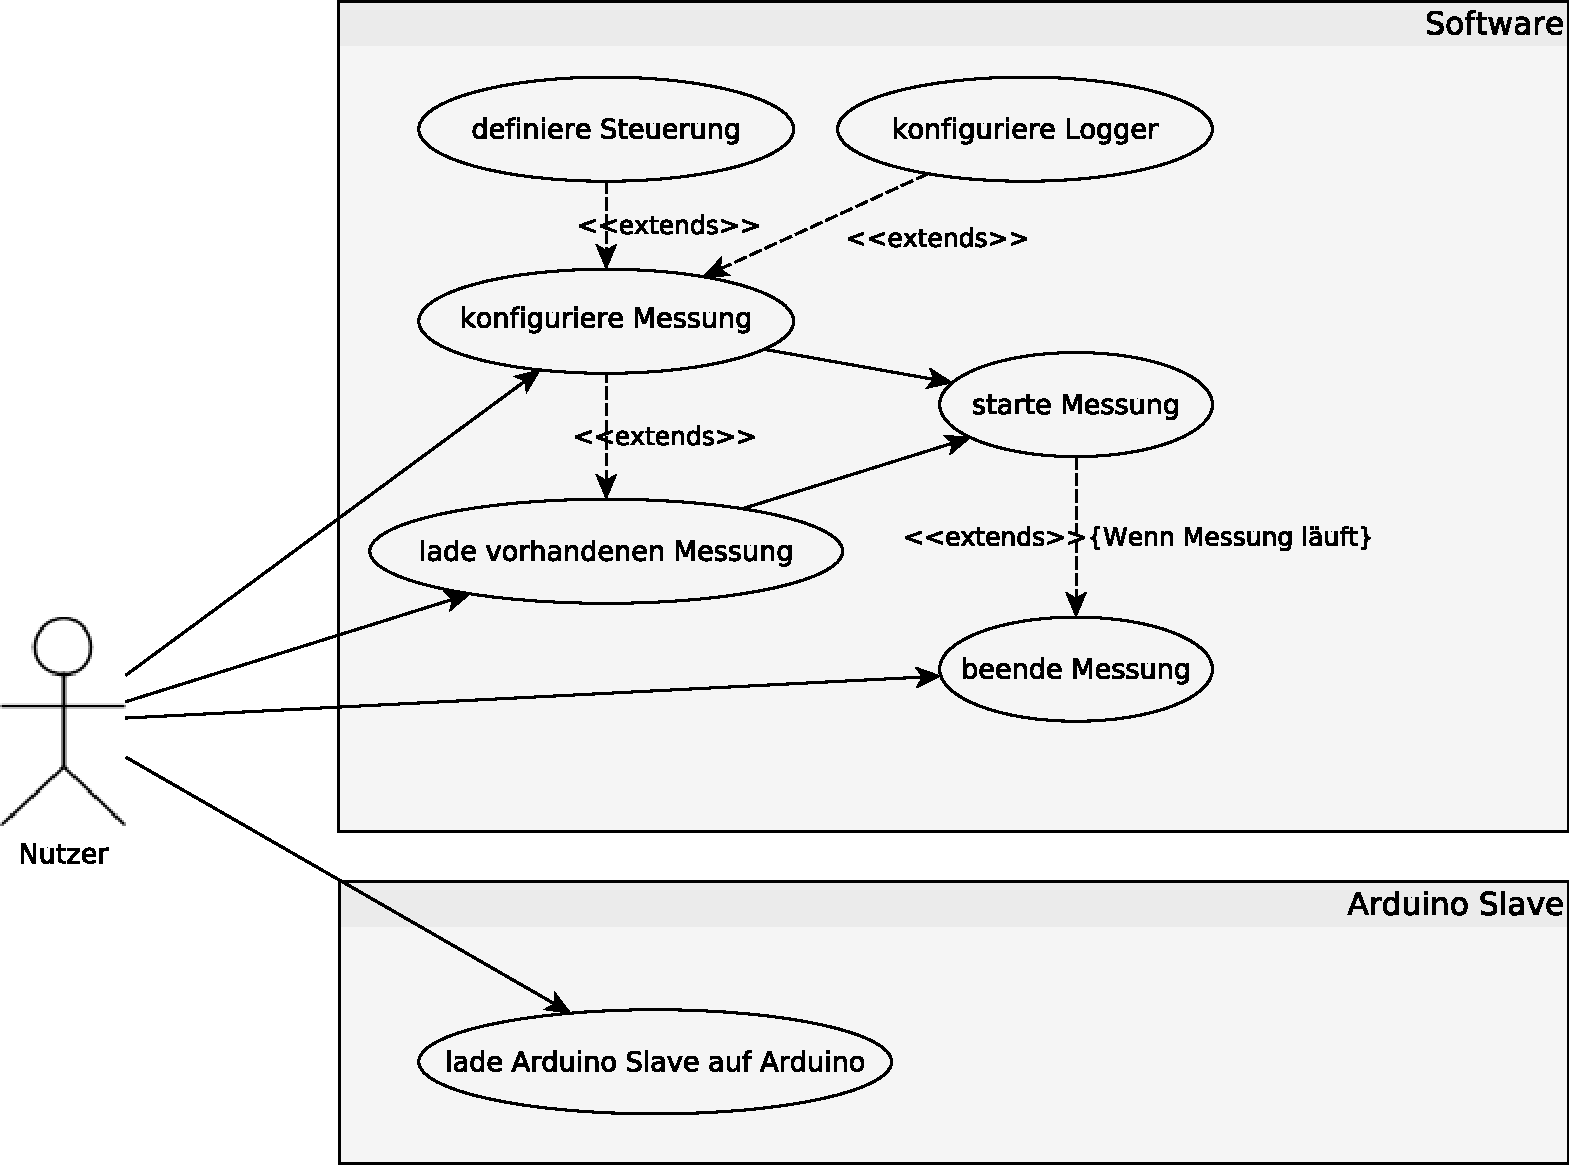
\includegraphics[width=\textwidth, keepaspectratio=true]{../Diagramme/BachelorUseCase1.pdf}
\end{figure}

%\section{Analysis object model}
%\section{Dynamic model}
\section{Flowchart}
Dieses Flowchart zeigt die notwendigsten Schritte, die von der Software und dem Nutzer unternommen werden müssen um eine erfolgreiche Messung durch führen zu können. 
\begin{figure}[H]
 \centering
 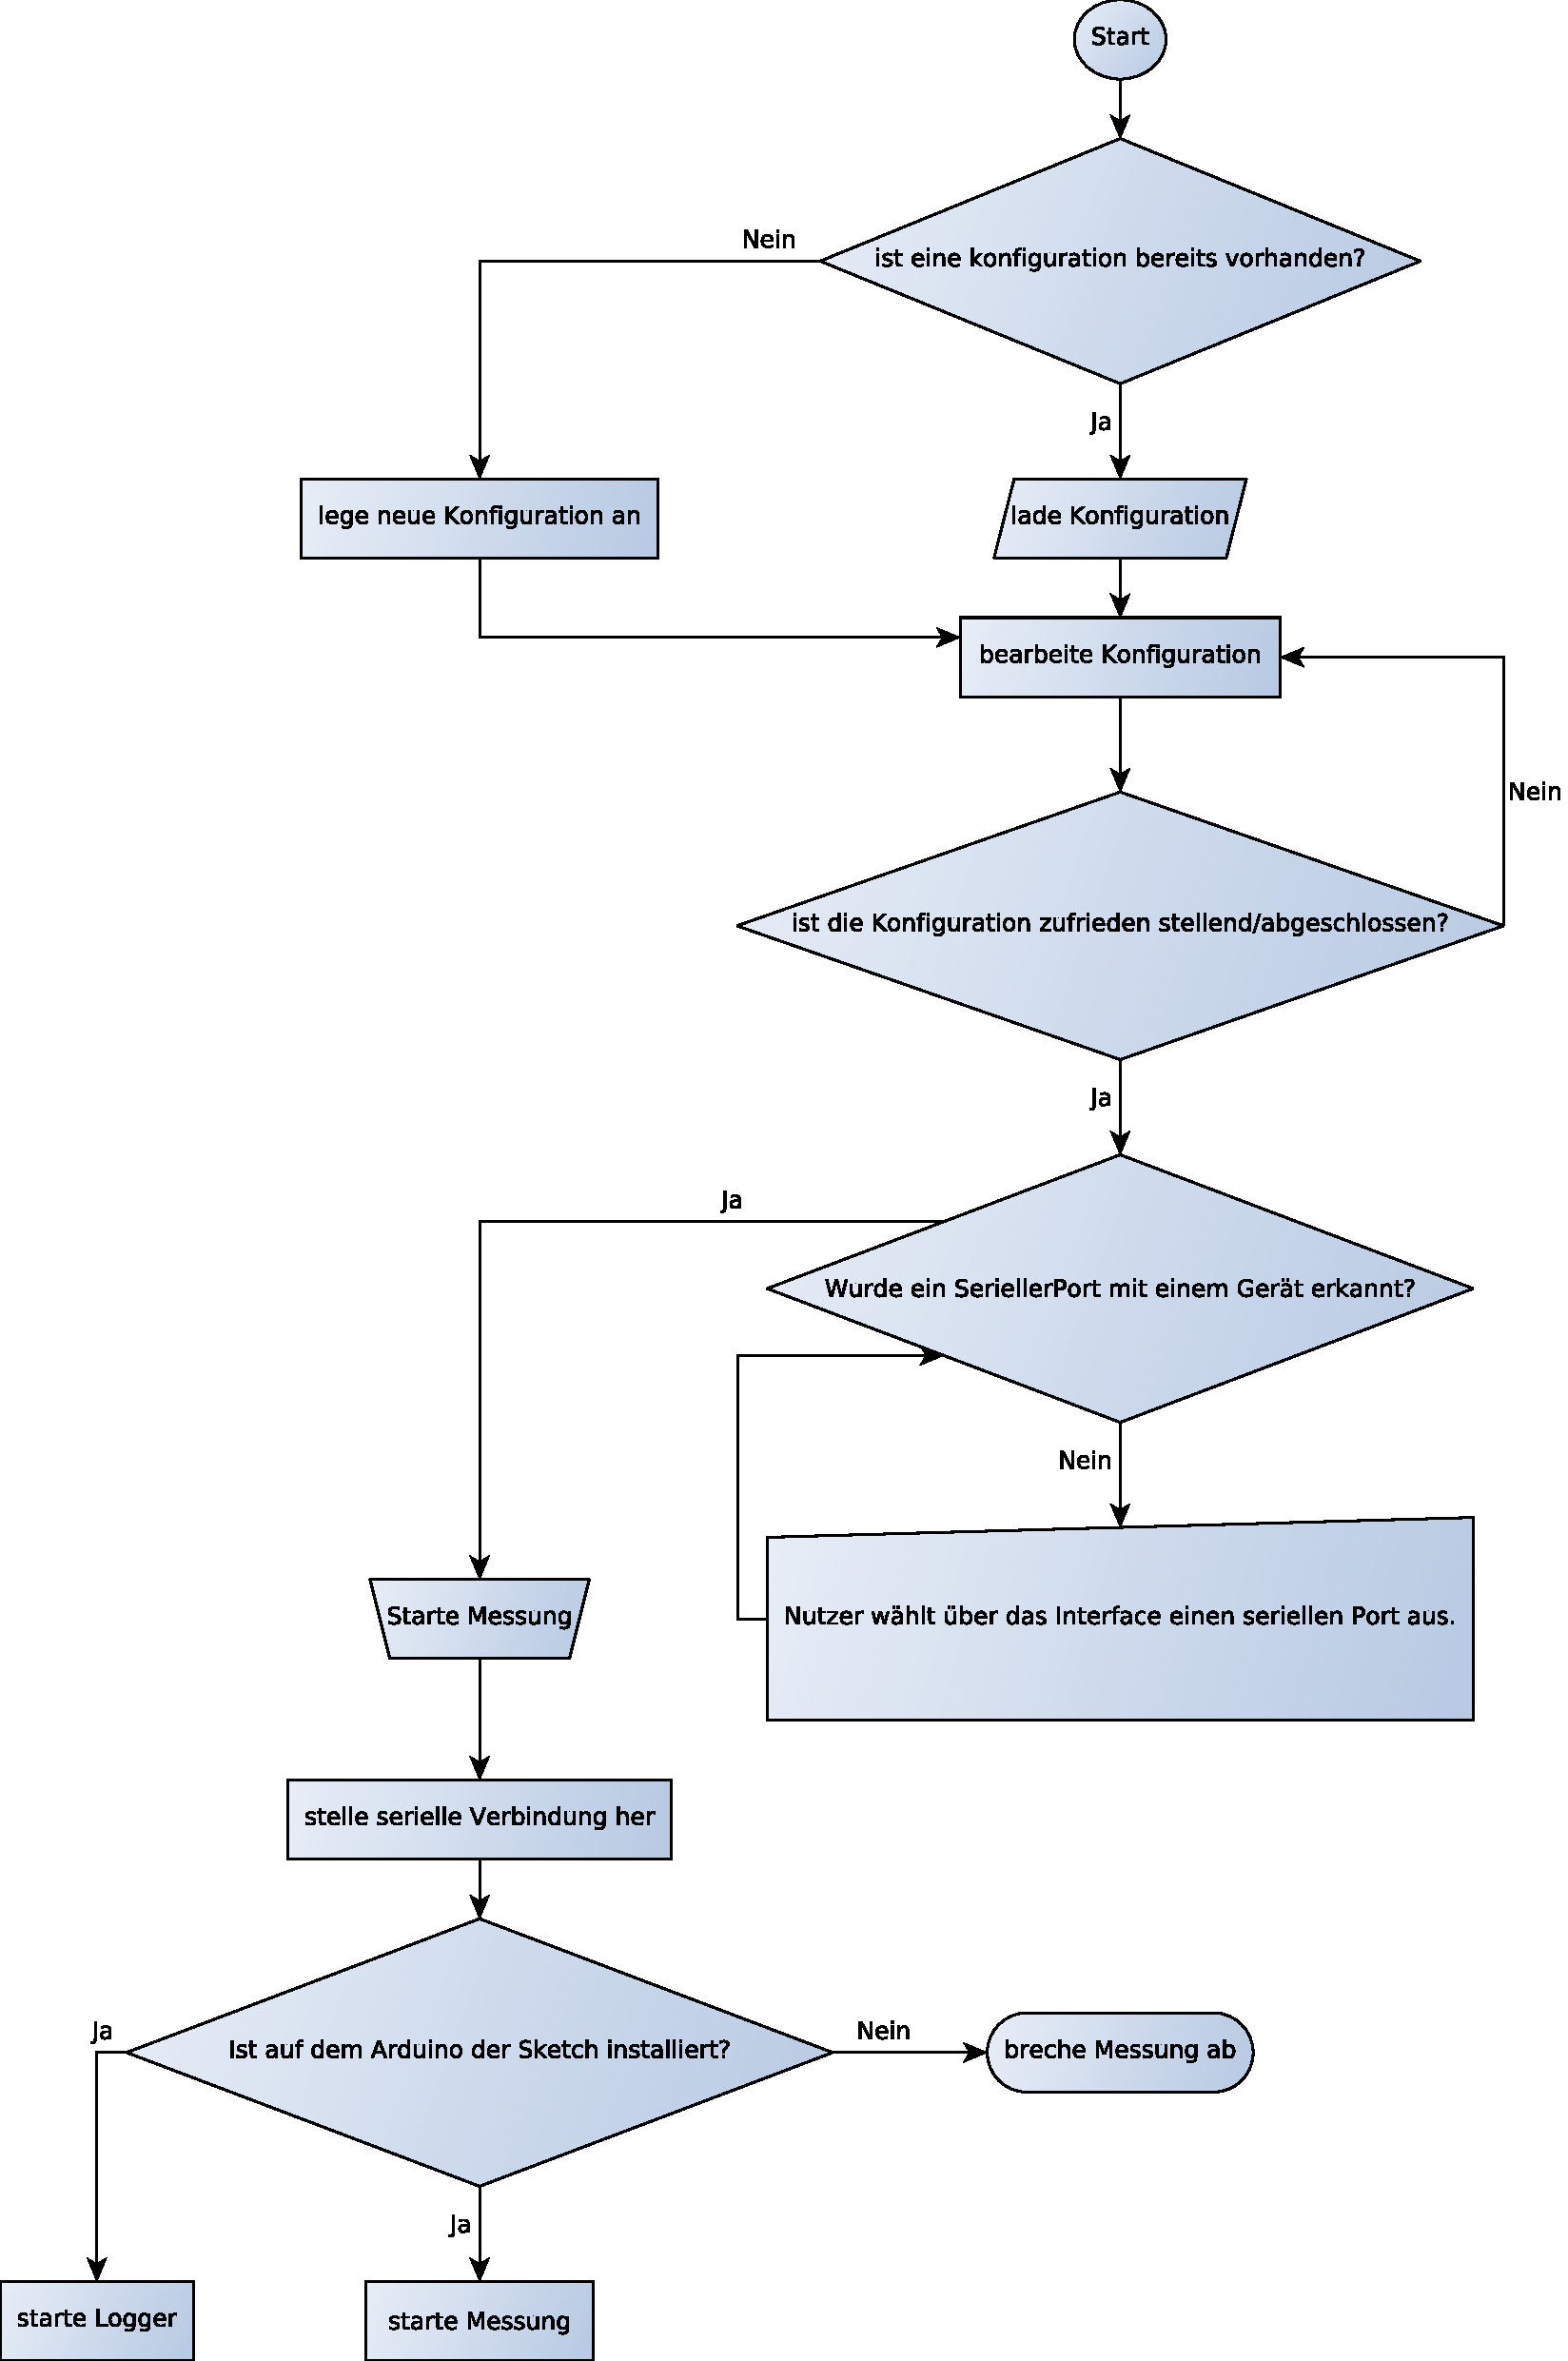
\includegraphics[width=\textwidth, keepaspectratio=true]{../Diagramme/SoftwareFlowChart.pdf}
\end{figure}
\section{Aufbau}
\begin{figure}[H]
 \centering
 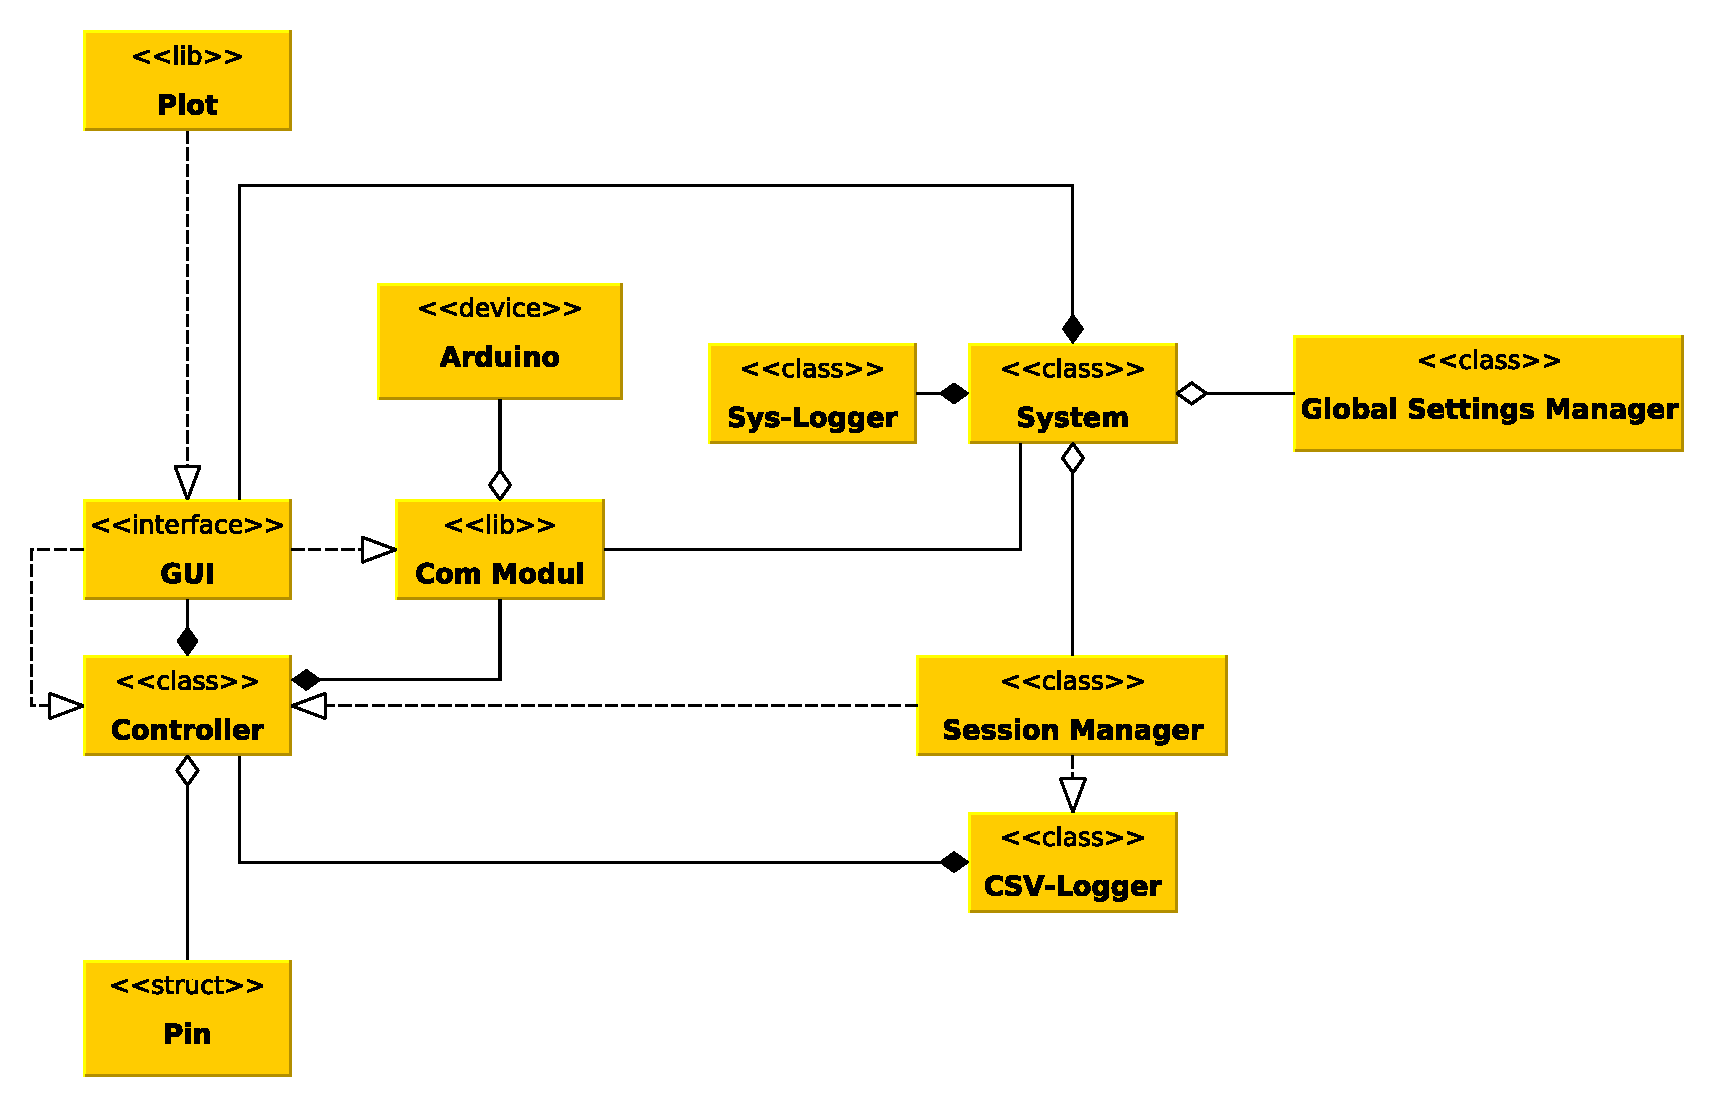
\includegraphics[width=\textwidth, keepaspectratio=true]{../Diagramme/StrukturUML.pdf}
\end{figure}
\section{User Interface - Wireframe}
Ein Wireframe befindet sich gerade noch in der Erarbeitungsphase und wird in einer späteren Version dieses Dokuments nachgereicht.